
\section{Database Layer}

\begin{enumerate}
\def\labelenumi{\arabic{enumi}.}
\itemsep1pt\parskip0pt\parsep0pt
\item
  Hibernate
\item
  Data Access Object
\item
  JAX-RS API 2.0
\end{enumerate}

\subsubsection{1. Hibernate}\label{hibernate}

Hibernate is an open source persistence and ORM framework for Java. It
is being used to map Java classes to database tables and provides means
to query and retrieve data without writing SQL.\\The mapping is done via
annotations which is being used for attributes as well as relations
between entities (many-to-one, many-to-many, etc.). In order for
Hibernate to manage the persistence, the class has to provide a no
arguments constructor. We used an extension to Hibernate called
Hibernate Spatial which also provides support for spatial data types
such as Point and MultiPolygon. Find an example below:


\begin{lstlisting}
@Id // indicating the primary key
@GeneratedValue(strategy=GenerationType.SEQUENCE) // how is the key generated
private long gid;

@Column(unique=true) // enforce unique constraint on column
private int wkr_nr;

// spatial type using extended annotations provided by hibernate spatial
@Type(type="org.hibernate.spatial.GeometryType")
@Column(columnDefinition="Geometry")
private Point centerPoint;

// ...

// defining a 1 <-> n relation between constituency and county
@OneToMany(fetch=FetchType.LAZY)
@JoinColumn(name="constituency_id", referencedColumnName="wkr_nr")
@OrderBy("areaQuota")
private List<CountyContainsConstituency> dependingCounties = new LinkedList<CountyContainsConstituency>();

// ...
\end{lstlisting}


\subsubsection{2. Data Access Object}\label{data-access-object}

\begin{figure}[htbp]
\centering
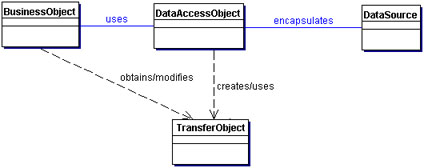
\includegraphics[width=0.9\textwidth]{../img/146804.jpg}
\caption{Data Access Object UML Diagram by Oracle (Core J2EE Patterns)}
\end{figure}

The pattern is used to provide a layer of abstraction between the actual
data source and the application logic using the data. By defining a
couple of interfaces and providing different implementing classes for
the different data sources changing the data source of an application
becomes rather easy. Below a UML diagram of our DAO classes.

\begin{figure}[htbp]
\centering
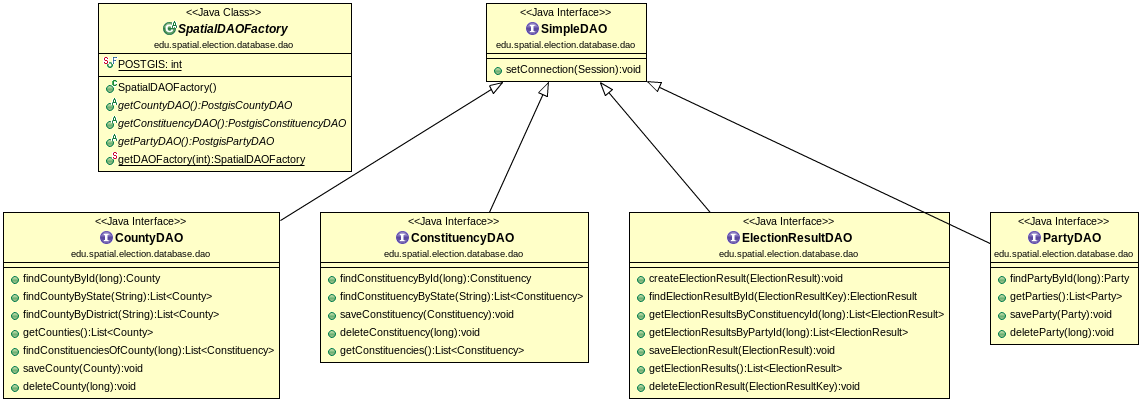
\includegraphics[width=1.2\textwidth]{../img/6CeJf06.png}
\caption{Class Diagramm}
\end{figure}

\textbf{Thoughts on using the pattern}\\Though it might seem a little
bit over the top to use such a rather complex structure for a small
scale project, we deemed it good software engineering practice to
separate data access from application logic. Moreover if a follow up
project wants to measure the performance of different databases while
using the application or simply decides to switch the underlying
database they simply need to implement another set of Data Access Object
classes.

\subsubsection{3. JAX-RS API 2.0}\label{jax-rs-api-2.0}

With the help of JAX-RS plain Java Objects can be exposed as RESTful Web
resources independent of the underlying technology using a declarative
and annotation based API.

\begin{lstlisting}
@Path("/constituency")
public class RestConstituency \{
    private SpatialDAOFactory f = SpatialDAOFactory.getDAOFactory(SpatialDAOFactory.POSTGIS);

	// ...
	
    @GET
    @Path("{id}/geometry")
    @Produces({MediaType.APPLICATION_JSON})
    public double[][][] getConstituencyGeometryById(@PathParam("id") long id)
    \{ Session s = DatabaseConnection.openSession();
        // Create a DAO
        ConstituencyDAO constituencyDAO = f.getConstituencyDAO();
        constituencyDAO.setConnection(s);

	Constituency c = constituencyDAO.findConstituencyById(id);
	c.setGeometryDetail(0);
	c.getGeometryArray();
	double[][][] result = c.getGeometryArray();
		
	s.close();
	return result;
    \}
    
	// ...
\}
\end{lstlisting}

\texttt{@Path} specifies the relative path of the function,
\texttt{@GET} the type of method (\texttt{@POST}, \texttt{@DELETE} and
\texttt{@PUT} are also available) and
\texttt{@Produces(\{MediaType.APPLICATION\_JSON\})} indicates that the
method will eventually return JSON (as opposed to \texttt{@Consumes}
which indicates that the method is passed a particular type).\\Another
interesting feature to note is \texttt{@PathParam} which is being passed
to the function. It's used to identify a single instance of a
constituency and binds the method parameter to a path segment.